\documentclass[SE,lsstdraft,authoryear,toc]{lsstdoc}
\input{meta}

% Package imports go here.

% Local commands go here.

%If you want glossaries
%\input{aglossary.tex}
%\makeglossaries

\title{PSF assessment in the field of Abell 360 and HSM shear profile using ComCam data.}

% This can write metadata into the PDF.
% Update keywords and author information as necessary.
\hypersetup{
    pdftitle={PSF assessment in the field of Abell 360 and HSM shear profile using ComCam data.},
    pdfauthor={First Last},
    pdfkeywords={}
}

% Optional subtitle
% \setDocSubtitle{A subtitle}

\author{%
First Last
}

\setDocRef{SITCOMTN-161}
\setDocUpstreamLocation{\url{https://github.com/lsst-sitcom/sitcomtn-161}}

\date{\vcsDate}

% Optional: name of the document's curator
% \setDocCurator{The Curator of this Document}

\setDocAbstract{%
The Rubin ComCam on-sky campaign performed at the end of 2024 provided observations of the Abell 360 galaxy cluster; these data allow a preliminary study of cluster weak lensing analysis using Rubin Data Preview 1 (DP1) data. Among all the steps required for such analyses, accurate modeling of the PSF is paramount. This work uses several diagnostics, mostly based on the residuals between the second moments of stars and the PSF model, to characterize the accuracy of the PSF modeling in the A360 field. We find the level of the residuals to be sufficiently low not to hinder the measurement of the tangential shear profile around A360.
}

% Change history defined here.
% Order: oldest first.
% Fields: VERSION, DATE, DESCRIPTION, OWNER NAME.
% See LPM-51 for version number policy.
\setDocChangeRecord{%
  \addtohist{1}{YYYY-MM-DD}{Unreleased.}{First Last}
}


\begin{document}

% Create the title page.
\maketitle
% Frequently for a technote we do not want a title page  uncomment this to remove the title page and changelog.
% use \mkshorttitle to remove the extra pages

% ADD CONTENT HERE
% You can also use the \input command to include several content files.

\section{Introduction}
The Rubin ComCam on-sky observing campaign (ref to SITCOMTN-149) undertaken at the end-of-year 2024 covered seven fields, among which the low ecliptic latitude Rubin SV 38 7 field. This field contains the Abell 360 (A360) galaxy cluster, an intermediate mass cluster ($M_{500,c} = 4.3\times 10^{14} \rm{M}_\odot$ from ACT DR5 SZ Cluster Catalog, ref) at z=0.22, that we use as a commissioning demonstrator of Rubin capabilities for cluster WL studies. This TechNote focuses on assessing the quality of the PSF modeling in the A360 field, as performed by the Rubin Science Pipeline for the Data Preview 1 (DP1) data release (ref to DP1 paper). PSF modeling was performed using the PSFex and Piff methods (Bertin et al., Jarvis et al.); the latter has been found more accurate (ref to the PSF section of DP1 paper, ref to PSTN-049 (https://pstn-019.lsst.io/PSTN-019.pdf), ref to LSST Science pipelines Papers) and has been used for the final modeling of DP1.

\section{Dataset}
The Rubin SV 38 7 field has been observed in $g$ (44 visits), $r$ (55 visits), $i$ (57 visits) and $z$ (27 visits) (ref to DP1 paper; ref to SITCOMTN-149; ref to RTN-095). No $u$ or $y$-band data were collected in that field. The $r$ or $i$-bands are generally used for weak lensing studies (ref to DES and HSC), the bluer bands being more affected by differential chromatic refraction (ref). For the DP1 analysis of A360 we will use the $i$-band, which received the most visits in DP1, to measure the shear profile around A360 and therefore focus on the $i$-band only for the purpose of this work. All the tests performed hereafter use data from the tracts and patches overlapping with  a 1 deg x 1 deg square field centered on the BCG of Abell 360, at (ra,dec) = (37.86, 6.98) deg. 
The DP1 object table gathers all the properties of the objects (stars and galaxies) detected in the coadded images, in each band. Figure XX shows the number of images that contributed to the coadds in the field of A360 and was obtained from the \code{i\_inputCount} information available in the object table. The dithering pattern of the observations is clearly visible.
%\includegraphics{Figures/nb_of_images.png}

\section{PSF properties and diagnostics}
\subsection{PSF residuals: whisker plots and distributions}
\begin{figure}
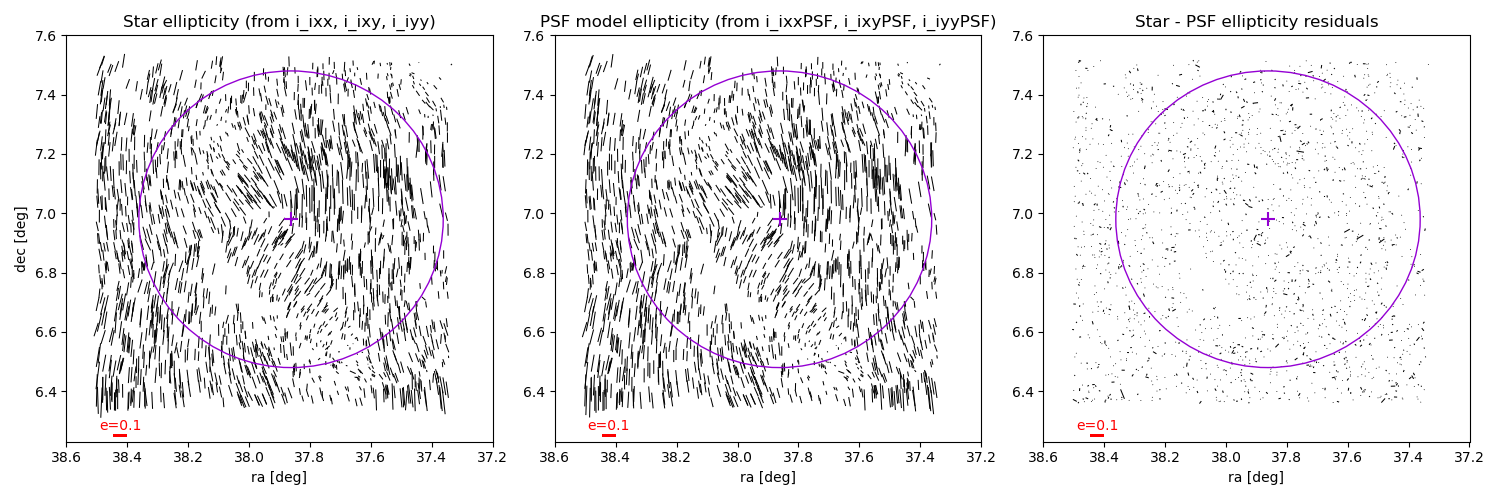
\includegraphics[width=\textwidth]{Figures/whiskers_used.png}
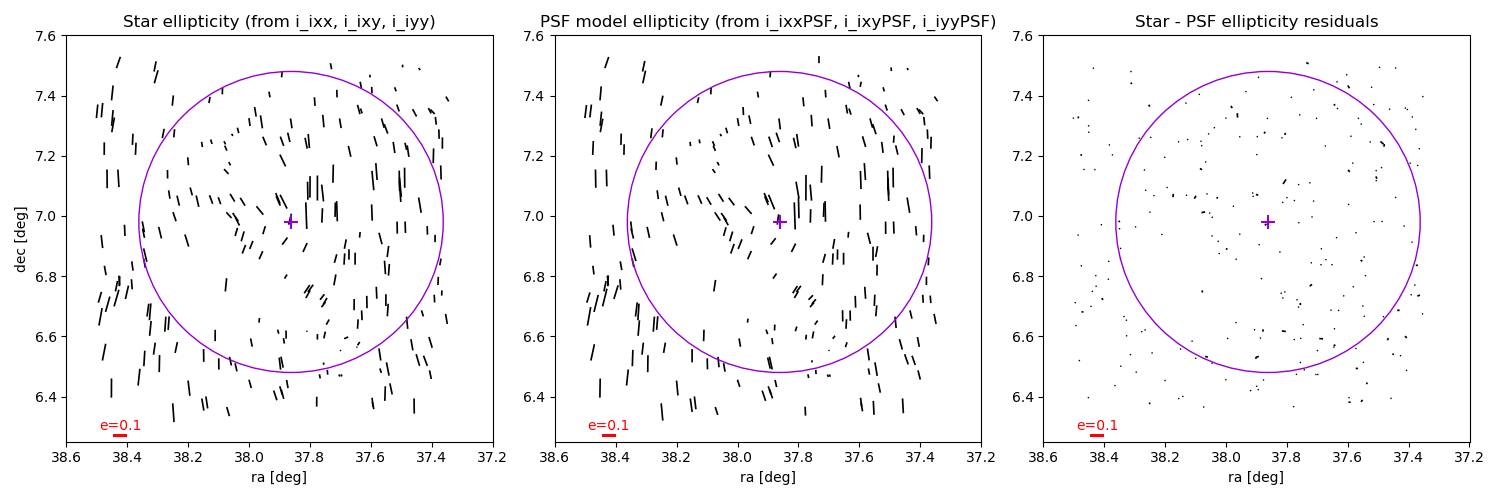
\includegraphics[width=\textwidth]{Figures/whiskers_reserved.png}
\caption{Whikser plots for the PSF (top) and reserved stars (bottom) obtained for the measurements (left), PSF model (middle) and the residuals (right). The size of the whiskers is proportional to the ellipticity modulus and the orientation gives the direction of the major exis of the ellipse. \label{fig:whiskers}}
\end{figure}
\subsection{PSF residuals - tangential shear profile}
\subsection{PSF rho-statistics}


\section{HSM tangential and cross shear profile around A360 from color-cut selection}

\appendix
% Include all the relevant bib files.
% https://lsst-texmf.lsst.io/lsstdoc.html#bibliographies
\section{References} \label{sec:bib}
\renewcommand{\refname}{} % Suppress default Bibliography section
\bibliography{local,lsst,lsst-dm,refs_ads,refs,books}

% Make sure lsst-texmf/bin/generateAcronyms.py is in your path
\section{Acronyms} \label{sec:acronyms}
\addtocounter{table}{-1}
\begin{longtable}{p{0.145\textwidth}p{0.8\textwidth}}\hline
\textbf{Acronym} & \textbf{Description}  \\\hline

DESC & Dark Energy Science Collaboration \\\hline
DM & Data Management \\\hline
DMTN & DM Technical Note \\\hline
DP1 & Data Preview 1 \\\hline
DRP & Data Release Processing \\\hline
HSC & Hyper Suprime-Cam \\\hline
HSM & Hierarchical Storage Management \\\hline
LSST & Legacy Survey of Space and Time (formerly Large Synoptic Survey Telescope) \\\hline
LSSTComCam & Rubin Commissioning Camera \\\hline
PSF & Point Spread Function \\\hline
RTN & Rubin Technical Note \\\hline
SE & System Engineering \\\hline
SNR & Signal to Noise Ratio \\\hline
SV & Science Validation \\\hline
TBC & To Be Confirmed \\\hline
USDF & United States Data Facility \\\hline
WL & Weak gravitational Lens cosmic shear \\\hline
\end{longtable}

% If you want glossary uncomment below -- comment out the two lines above
%\printglossaries





\end{document}
